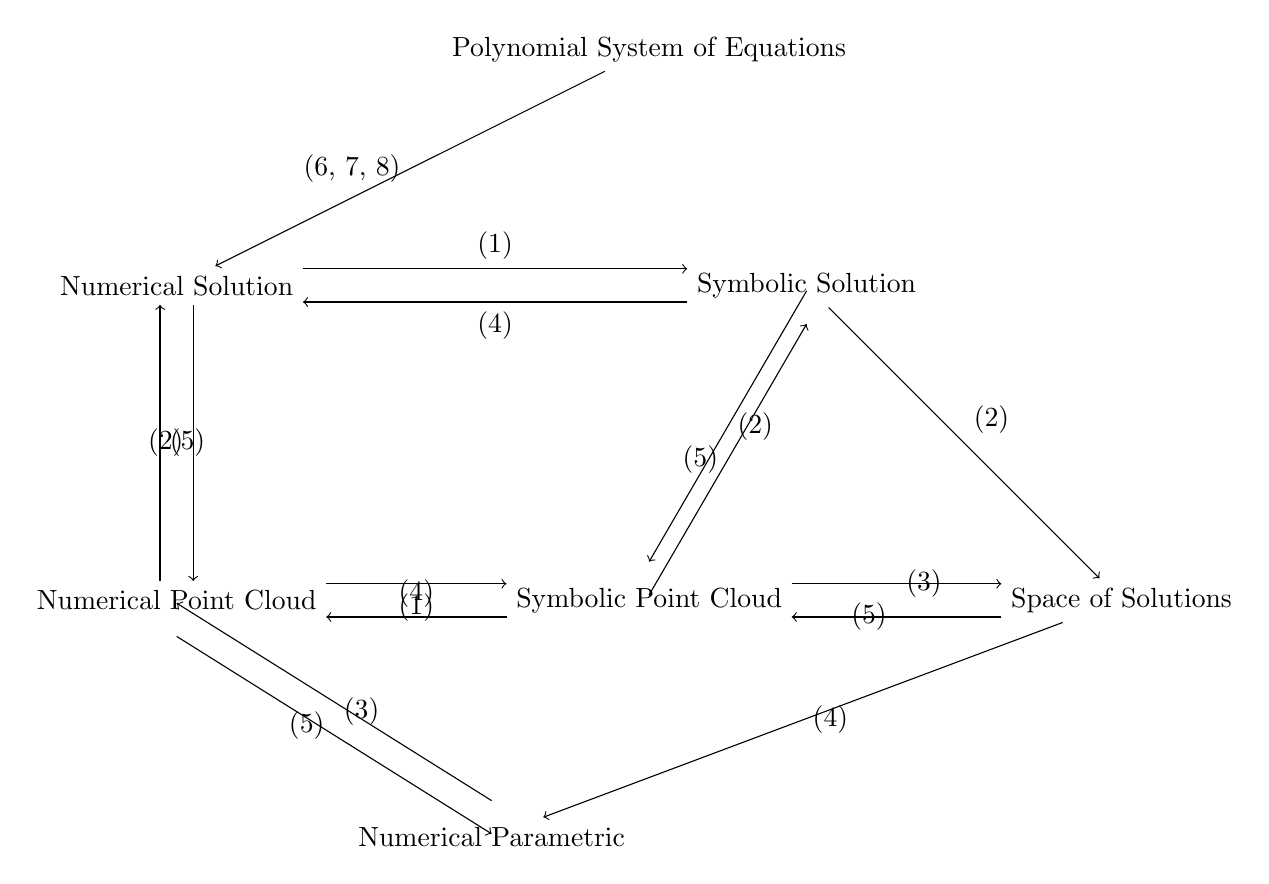
\begin{tikzpicture}[node distance=2cm]
  % spread out layout
  \node (start) at (6,0) {Polynomial System of Equations};
  \node (numerical) at (0,-3) {Numerical Solution};
  \node (symbolic) at (8,-3) {Symbolic Solution};
  \node (num_cloud) at (0,-7) {Numerical Point Cloud};
  \node (sym_cloud) at (6,-7) {Symbolic Point Cloud};
  \node (parametric) at (12,-7) {Space of Solutions};
  \node (num_parametric) at (4,-10) {Numerical Parametric};

  % Straight arrows (no bends)
  \draw[->] (start) -- (numerical) node[midway, left] {(6, 7, 8)};
  \draw[->] ([yshift=6pt]numerical.east) -- ([yshift=6pt]symbolic.west) node[midway, above] {(1)};
  \draw[->] ([yshift=-6pt]symbolic.west) -- ([yshift=-6pt]numerical.east) node[midway, below] {(4)};
  \draw[->] ([xshift=6pt]numerical.south) -- ([xshift=6pt]num_cloud.north) node[midway, left] {(2)};
  \draw[->] ([yshift=6pt]symbolic.south) -- ([yshift=6pt]sym_cloud.north) node[midway, right] {(2)};
  \draw[->] ([xshift=-6pt]num_cloud.north) -- ([xshift=-6pt]numerical.south) node[midway, right] {(5)};
  \draw[->] ([yshift=-6pt]sym_cloud.north) -- ([yshift=-6pt]symbolic.south) node[midway, left] {(5)};
  \draw[->] ([yshift=6pt]num_cloud.east) -- ([yshift=6pt]sym_cloud.west) node[midway, below] {(1)};
  \draw[->] ([yshift=-6pt]sym_cloud.west) -- ([yshift=-6pt]num_cloud.east) node[midway, above] {(4)};
  \draw[->] ([yshift=6pt]sym_cloud.east) -- ([yshift=6pt]parametric.west) node[midway, right] {(3)};
  \draw[->] ([yshift=-6pt]parametric.west) -- ([yshift=-6pt]sym_cloud.east) node[midway, left] {(5)};
  \draw[->] (symbolic) -- (parametric) node[midway, above right] {(2)};
  \draw[->] (parametric) -- (num_parametric) node[midway, right] {(4)};
  \draw[->] ([yshift=6pt]num_parametric.north) -- ([yshift=6pt]num_cloud.south) node[midway, below left] {(5)};
  \draw[->] ([yshift=-6pt]num_cloud.south) -- ([yshift=-6pt]num_parametric.north) node[midway, above right] {(3)};
\end{tikzpicture}
